\begin{surferPage}[Cono Doppio]{Un Cono Doppio}
Come spiegato nell'introduzione a questa galleria, una superficie \`e detta \emph{non-singolare} o \emph{liscia} se non ha punte (le punte sono dette \emph{singolarit\`a\/}).

Per esempio, una sfera o un toro (le due figure a sinistra qui sotto):
    \begin{center}
      \begin{tabular}{@{}c@{}c@{}c@{}c@{}}
        \begin{tabular}{@{}c}
          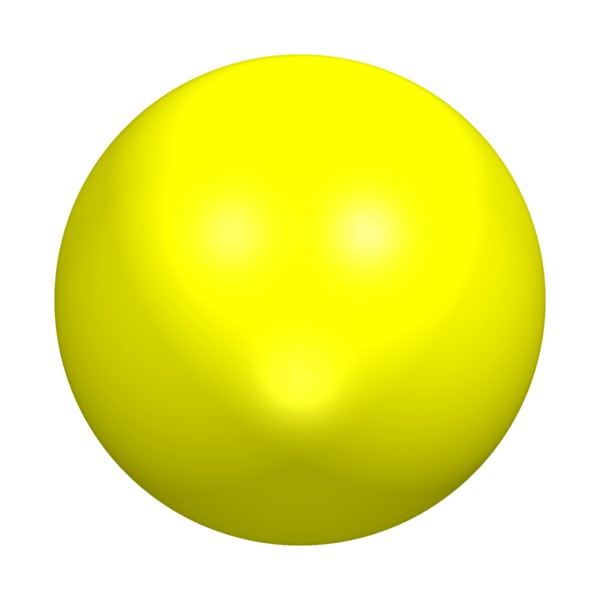
\includegraphics[width=1.4cm]{kugel}
        \end{tabular}
        &
        \begin{tabular}{@{}c}
          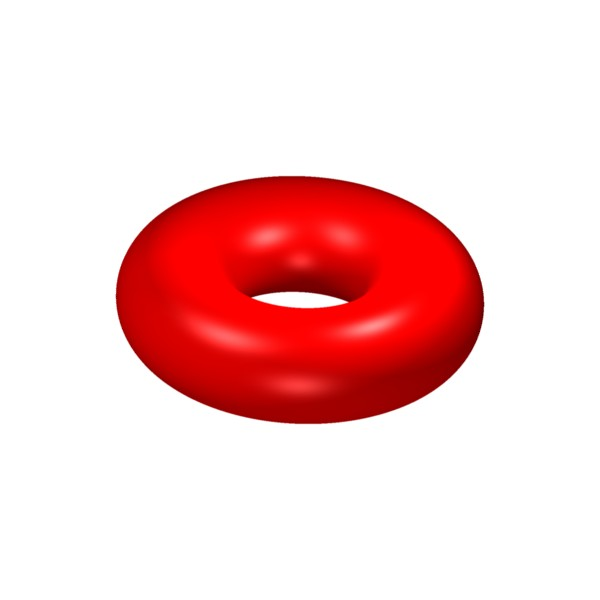
\includegraphics[width=1.4cm]{torus}
        \end{tabular}
        &
        \begin{tabular}{c@{}}
          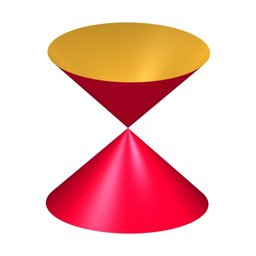
\includegraphics[width=1.4cm]{kegel}
        \end{tabular}
      \end{tabular}
    \end{center}
    Il cono doppio (figura a destra) \`e la singolarit\`a pi\`u semplice; \`e l'unica singolarit\`a che pu\`o essere descritta da un'equazione di grado $2$:
    \[x^2+y^2-z^2=0.\]
    Se modifichiamo leggermente questa equazione sostituendo lo $0$ con un valore piccolo $a\neq 0$, il cono doppio si trasforma in uno dei due tipi di iperboloide, a seconda del segno di $a$:
    \begin{center}
      \begin{tabular}{@{}c@{\ }c@{\ }c@{\ }c@{\ }c@{}}
        \begin{tabular}{@{}c@{}}
          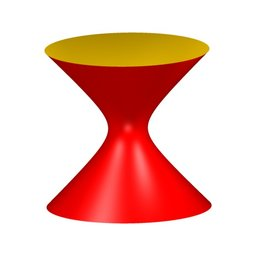
\includegraphics[width=1.2cm]{A1pm_2}
        \end{tabular}
        &
        $\leftarrow$
        &
        \begin{tabular}{@{}c@{}}
          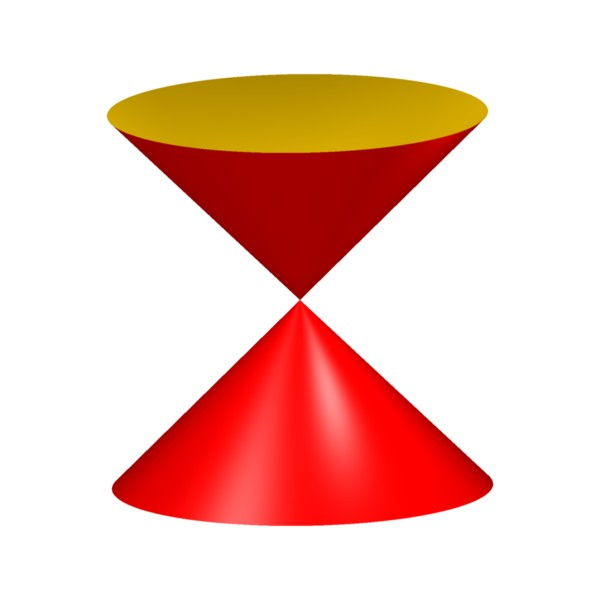
\includegraphics[width=1.2cm]{A1pm_1} 
        \end{tabular}
        &
        $\rightarrow$
        &
        \begin{tabular}{@{}c@{}}
          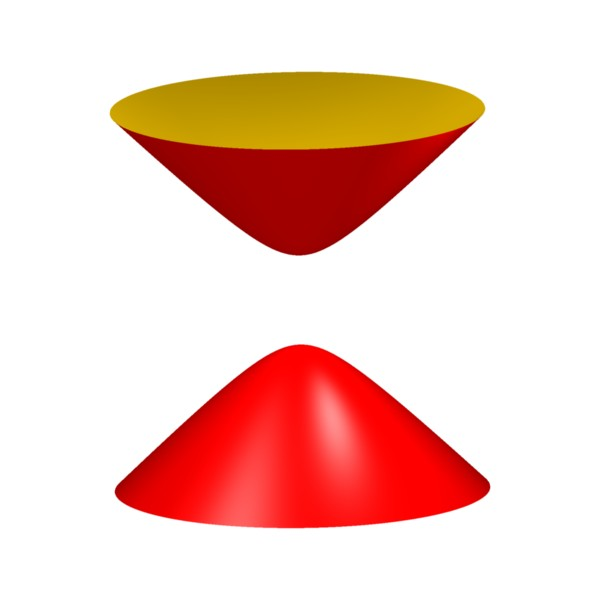
\includegraphics[width=1.2cm]{A1pm_0}
        \end{tabular}
      \end{tabular}
    \end{center}
   Una superficie di grado $2$ non pu\`o avere pi\`u di una singolarit\`a, ossia $\mu(2)=1$.
\end{surferPage}
